\documentclass{ltjsarticle}
\usepackage{amsmath}
\usepackage{tikz}
% TikZの拡張ライブラリ（図形、矢印の形、相対配置、計算）を読み込む

\usetikzlibrary{shapes.geometric, arrows.meta, positioning, calc}


\title{今よりもちょっと良いLEDドライバを作ろう}
\author{飯田健登\thanks{https://mathlandscape.com/}}
\date{2026年6月11日}
\begin{document}
\maketitle

\section{はじめに}
本稿では、後継のLEDドライブ基板への採用を目指して、『今よりもちょっと良い外観検査向けLEDドライバ』を提案する。
外観検査向けLEDドライバはカメラの露光タイミングと同期して、電圧もしくは電流値の高い再現性があることや低遅延かつ低ジッタで動作することが要求される。
またコスト面でも、より少ない部品点数かつ狭い実装面積で製作できるかが重要である。
また、調光の制御方式としていくつか挙げられるが、市販製品の多くはLEDに一定電圧(24Vなど)を印可し、PWM調光を行うものである。
開ループ制御であるため高速かつ安定した出力が可能であり、また、回路構成もシンプルなため安価に製作可能である。
しかし、露光中に一定周期で点灯→消灯→点灯...と繰り返すため、ローリングシャッターのカメラでは画像内で明るさムラ（縞模様）が発生してしまう他、
グローバルシャッターのカメラであっても、PWM周波数に対して露光時間が短い場合には、画像間の明るさにちらつきが発生が懸念される。

弊社の多くの内製外観検査設備では、電流アナログ調光方式を採用している。露光中はプリセットした一定の電流を連続的に出力するため、
先述した明るさムラやちらつきの発生リスクが大幅に少なく、電流とLEDの明るさとの関係は概ね線形であるため、直感的に調光できるといった利点が挙げられる。
ただし、PWM制御方式と異なり閉ループ制御であるためコントローラー設計次第で、照明ケーブルやLED負荷による位相遅れを十分に補正できず、発振が起こってしまうリスクを抱えている。
内製設備では、アナログ回路のフィードバック制御による定電流回路を搭載したDR-X-147やDR-CY-140、あるいはこれらと互換性のある先代の基板が多く採用されているが、
一定以上照明ケーブルを長くした場合や電源電圧に対してLEDの順方向電圧が著しく小さい場合などで発振が起こる場合がある。
とはいうものの、現行のLEDドライバでも発振が起こらないようにある程度の位相補償がなされている。ここでの位相補償の方式は、フィードバックループのループゲインを抑えることで
発振条件を満たさないようにするものであり、効果的に発振を抑えることができる反面、速応性が低下してしまうことが知られている。
現行回路では、速応性を優先して、安定性の観点では位相補償が十分でないため、実際に一部の設備では発振が起こることが確認されている。

そこで、本稿では、現行の回路で採用されている回路トポロジーを理解し、発振が起こる要因や改善点を明らかにする。
その上で、新たな回路トポロジーを提案するとともに、速応性を可能な限り維持しつつ、十分な安定性を確保した位相補償の方式について検討し、
速応性と安定性の両面から従来回路との提案回路との比較・評価を行う。

\section{現行LEDドライバーの動作機構を理解しよう}

本章では、現行のLEDドライブ回路の動作機構を理解するとともに、現状起こっている発振やその対策、今後改善すべき課題を明らかにする。
\subsection{現行LEDドライブ回路の動作機構}
DY-CY-140,DR-X-147のLEDドライブ回路を図に示す。
いずれの回路も細かい点で違いは見られるが、共通のトポロジーを持つ回路である。
図に記した通り、この回路は大きく分けて前段と後段に分けられる。
前段回路は目標値（電圧）を電源電圧から目標値を差し引いた電圧に変換する機構を持っている。
一方で後段回路は前段回路で作られた電圧指令値を入力として、これを基にLEDに流れる電流が駆動される。

直流解析でさらに詳しく動作機構を解説する。
DR-X-147の回路をもとに説明する。
図中の$DAC  OUT0$が目標値入力、$VDD1$〜$VDD3$が電源、$LED_CH0$が電流出力である。
$DAC  OUT0$から目標値$V_{ref}$をオペアンプU3Aの非反転入力端子に入力すると、定常状態では反転入力端子も同電位となるため、
$R39$に両端電圧は$V_{ref}$と等しくなる。
このとき、エミッタ電流$I_{E}$は$\frac{V_{ref}}{2000}$となるため、トランジスタ$Q4$のコレクタ電圧$V_{C}$は

\begin{equation}
    V_{C} = V_{DD} - \frac{V_{ref}}{2000} \cdot (560 + 470)
\end{equation}

$V_{C}$は後段回路のオペアンプの非反転入力端子に接続され、同様に定常状態では反転入力端子の電位と同電位となる。
反転入力端子の電位は次のように表せる。


\begin{equation}
    V_{-} = \frac{V_{dd} - R_{64}I}{R_{46}+R_{49}} \cdot R_{46}
\end{equation}




%動作機構の解説
 %電流吐き出し型の定電流回路が採用される
 %直流解析
 %ラプラス変換　伝達関数モデル
\subsection{なぜ発振が起こるのか？}

\subsection{発振を抑えるには？またその課題は？}
%課題・改善点


\section{提案するLEDドライバーの動作機構と位相補償について理解しよう}

%直流解析
%ラプラス変換によるモデル化　伝達関数

図1に示すオペアンプU1の非反転入力端子の電位を$v_{+}(t)$とするとき、次式で示せる。
\begin{equation}
v_{+}(t) = V_{ref} + R(i_{c}(t) + i_{R}(t))
\end{equation}

また、トランジスタQ1のコレクタ電圧を$v_{o}(t)$とするとき、$i_{c}(t)$および$i_{c}(t)$は次のように示せる。
\begin{gather}
\frac{1}{C} \int i_{c}(t) \, dt = v_{o}(t) - v_{+}(t) \\
i_{R}(t) = \frac{v_{o}(t) - v_{+}(t)}{kR}
\end{gather}

式(1)、式(2)および(3)の両辺をラプラス変換すると、以下の式を得る。

\begin{gather}
    V_{+}(s) = V_{ref} + R(I_{c}(s) + I_{R}(s)) \\
    \frac{I_{c}(s)}{sC} = V_{o}(s) - V_{+}(s) \\
    I_{R}(s) = \frac{V_{o}(s) - V_{+}(s)}{kR}
\end{gather}

式(4)に式(5)、(6)を代入すると、以下の式を得る。

\begin{gather*}
\begin{aligned}
    V_{+}(s) &= V_{ref} + R\{Cs(V_{o}(s) -  V_{+}(s)) + \frac{V_{o}(s) - V_{+}(s)}{kR}\} \\
    &= V_{ref} + CRs(V_{o}(s) -  V_{+}(s)) + \frac{V_{o}(s) - V_{+}(s)}{k}
\end{aligned}
\end{gather*}

\begin{equation*}
    \Rightarrow V_{+}(s)(CRs+1+\frac{1}{k}) = V_{ref} + V_{o}(s)(CRS+\frac{1}{k})
\end{equation*}

\begin{equation}
    V_{+}(s) = \frac{V_{ref}+V_{o}(s)(CRs + \frac{1}{k})}{CRs + 1+ \frac{1}{k}}
\end{equation}

同様に、反転入力端子の電位を$v_{-}(t)$とするとき、次式で示せる。
\begin{equation}
    v_{-}(t) = \frac{1}{k+1}V_{cc}
\end{equation}
両辺ラプラス変換すると、
\begin{equation}
    V_{-}(s) = \frac{1}{k+1}V_{cc}
\end{equation}

オペアンプの開ループ伝達関数を$A(s)$とするとき、オペアンプの出力電圧$V_{op}(s)$は次のように示せる。
\begin{gather*}
    \begin{aligned}
    V_{op}(s) &= A(s)(V_{+}(s) - V_{-}(s)) \\
    &=A(s)\{\frac{V_{ref} + V_{o}(s)(CRs + \frac{1}{k})}{CRs + 1+ \frac{1}{k}} - \frac{V_{cc}}{k+1}\} \\
    &=A(s)\{\frac{(k+1)V_{ref} + V_{o}(s)(kCRs + CRs + 1 + \frac{1}{k}) - V_{cc}(CRs + 1 + \frac{1}{k})}{(k+1)CRs+(k + \frac{1}{k} + 2)}\} \\
    &V_{o}(s) = V_{cc} - R_{s}I(s)より、\\
    &=A(s)\{\frac{(k+1)V_{ref} + (V_{cc} - R_{s}I(s))(kCRs + CRs + 1 + \frac{1}{k}) - V_{cc}(CRs + 1 + \frac{1}{k})}{(k+1)CRs+(k + \frac{1}{k} + 2)}\} \\
    &=A(s)\{\frac{(k+1)V_{ref} + kV_{cc}CRs - R_{s}I(s)(kCRs+CRs+1+\frac{1}{k})}{(k+1)CRs + \frac{1}{k}(k+1)^2} \} \\
    &=A(s)\{\frac{(k+1)V_{ref} + kV_{cc}CRs - R_{s}I(s)\frac{k+1}{k}(kCRs+1)}{(k+1)CRs + \frac{1}{k}(k+1)^2} \} \\
    &=A(s)\{\frac{V_{ref} + \frac{k}{k+1}V_{cc}CRs-R_{s}I(s)(CRs+\frac{1}{k})}{CRs + \frac{k+1}{k}}\} \\
    &\frac{k}{k+1}V_{cc}CRは変動せず一定(時間微分すると0)のため、\frac{k}{k+1}V_{cc}CRs = 0 \\
    &=A(s)\{\frac{V_{ref}-R_{s}I(s)(CRs+\frac{1}{k})}{CRs + \frac{k+1}{k}}\} \\
    &=\frac{k}{k+1}A(s)\{\frac{V_{ref}-R_{s}I(s)(CRs+\frac{1}{k})}{1 + \frac{k}{k+1}CRs}\}
    \end{aligned}
\end{gather*}
LED照明やトランジスタQ1を含む制御対象を$G(s)$として、ブロック線図に展開すると、図2のようになる。\\


%ここにブロック線図を書く




\begin{center}
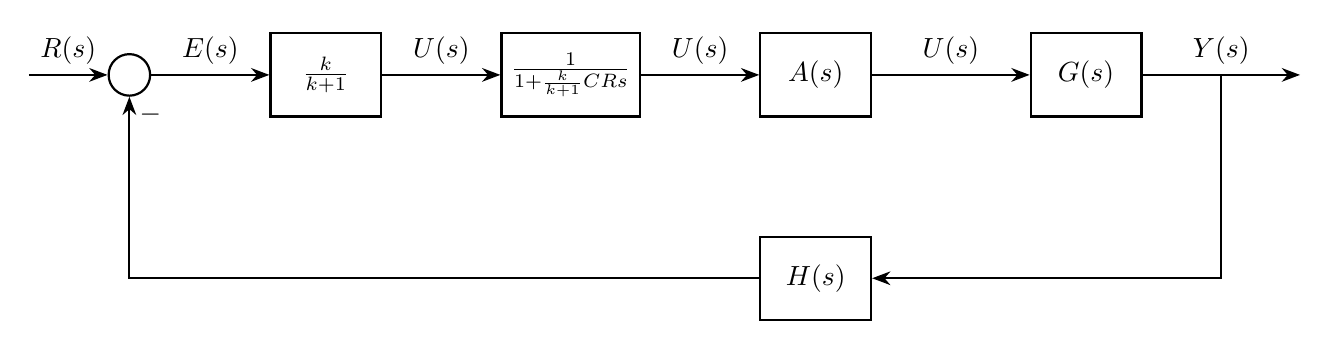
\begin{tikzpicture}[
    auto,
    node distance=2cm,
    >=Stealth, % 矢印の形
    % ブロックの基本デザインを定義
    block/.style={rectangle, draw, thick, minimum height=3em, minimum width=4em, font=\sffamily},
    % 突き合わせ点（丸）のデザインを定義
    sum/.style={circle, draw, thick, minimum size=1.5em, inner sep=0pt},
    % 線の端点の見えない要素
    coord/.style={coordinate}
]

% 1. 各要素（ノード）の配置
\node [coord] (input) {};
\node [sum, right=1.0cm of input] (sum1) {};
\node [block, right=1.5cm of sum1] (P_block) {$\frac{k}{k+1}$};
\node [block, right=1.5cm of P_block] (first_order_system) {$\frac{1}{1+\frac{k}{k+1}CRs}$};
\node [block, right=1.5cm of first_order_system] (OpAmp) {$A(s)$};
\node [block, right=2cm of OpAmp] (Target) {$G(s)$};
\node [coord, right=2cm of Target] (output) {};

\node [block, below=1.5cm of OpAmp] (feedback_block) {$H(s)$};

% 2. 要素同士を線（矢印）で結ぶ
\draw [->, thick] (input) -- node {$R(s)$} (sum1);
\draw [->, thick] (sum1) -- node {$E(s)$} (P_block);
\draw [->, thick] (P_block) -- node {$U(s)$} (first_order_system);
\draw [->, thick] (first_order_system) -- node {$U(s)$} (OpAmp);
\draw [->, thick] (OpAmp) -- node {$U(s)$} (Target);
\draw [->, thick] (Target) -- node[name=y] {$Y(s)$} (output);

% 3. フィードバックループを描く
% 出力Y(s)の途中から下へ線を下ろし、左へ進んで、足し合わせ点の下へ繋ぐ
\draw [->, thick] (y) |- (feedback_block);
% フィードバックブロックから左へ進み、上へ上がって足し合わせ点(sum1)の下へ繋ぐ
\draw [->, thick] (feedback_block) -| node[pos=0.95, right] {$-$} (sum1.south);

\end{tikzpicture}
\end{center}



次にオペアンプの出力と反転入力端子との間に位相補償キャパシタを接続した場合を考える。
非反転入力端子の電圧$v_{+}(t)$は次のように示せる。
\begin{equation}
    v_{+}(t) = V_{ref} + i_{R}(t) \cdot R
\end{equation}

\begin{equation*}
    i_{R}(t)=\frac{v_{o}(t)-V_{ref}}{(k+1)R} より、
\end{equation*}

\begin{equation}
    v_{+}(t) = V_{ref} + \frac{v_{o}(t)-V_{ref}}{(k+1)}
\end{equation}
両辺をラプラス変換すると、
\begin{equation}
    V_{+}(s) = V_{ref} + \frac{V_{o}(s)-V_{ref}}{(k+1)}
\end{equation}

反転入力端子の電圧$V_{-}(s)$は次のように示せる。
\begin{equation}
        v_{-}(t) = \{\frac{V_{cc}}{(k+1)R} + i_{c}(t)\}R
\end{equation}
両辺をラプラス変換すると
\begin{equation}
        V_{-}(s) = \{\frac{V_{cc}}{(k+1)R} + I_{c}(s)\}R
\end{equation}


\begin{equation}
    \frac{1}{C} \int i_{c}(t) \, dt = v_{op}(t) - v_{-}(t)
\end{equation}

両辺ラプラス変換すると、
\begin{gather}
    \frac{1}{sC} I_{c}(s) = V_{op}(s) - V_{-}(s) \\
    \Rightarrow I_{c}(s) = sC\{V_{op}(s) - V_{-}(s)\}
\end{gather}

式(14)に代入すると、
\begin{equation}
    \begin{aligned}
        V_{-}(s) &= \{\frac{V_{cc}}{(k+1)R} + sC(V_{op}(s) - V_{-}(s))\}R \\
        &= \frac{\frac{V_{cc}}{k+1} + CRsV_{op}(s)}{1+CRs}
    \end{aligned}
\end{equation}


\begin{gather*}
    \begin{aligned}
        V_{op}(s) &= A(s)(V_{+}(s) - V_{-}(s)) \\
        &= A(s) \{\frac{V_{o}(s)}{k+1} + V_{ref} \cdot \frac{k}{k+1} -  \frac{\frac{V_{cc}}{k+1} + CRsV_{op}(s)}{1+CRs}\} \\
        &= A(s) \{\frac{V_{o}(s) + kV_{ref}}{k+1} -  \frac{\frac{V_{cc}}{k+1} + CRsV_{op}(s)}{1+CRs}\} \\
        &= A(s) \{\frac{(V_{o}(s) + kV_{ref})(1+sCR) - V_{cc} - (k+1)CRsV_{op}(s)}{(k+1)(1+sCR)}\} \\\\
        &V_{o}(s) = V{cc} - R_{s}I(s)より \\
        &= A(s) \{\frac{(V{cc} - R_{s}I(s) + kV_{ref})(1+sCR) - V_{cc} - (k+1)CRsV_{op}(s)}{(k+1)(1+sCR)}\} \\
        &= A(s) \{\frac{CRsV_{cc}-R_{s}I(s)-CRsR_{s}I(s)+kV_{ref}+sCRkV_{ref}-(k+1)CRsV_{op}(s)}{(k+1)(1+sCR)}\}
    \end{aligned}
\end{gather*}


\begin{gather*}
    \begin{aligned}
        \Rightarrow V_{op}(s)\{1+\frac{CRs}{1+CRs} \cdot A(s) \} &= A(s)\{\frac{-R_{s}I(s)-sCRR_{s}I(s)+kV_{ref}(1+CRs)}{(k+1)(1+sCR)} \} \\
        &= A(s)({\frac{kV_{ref}-R_{s}I(s)}{k+1}})
    \end{aligned}
\end{gather*}


\begin{gather*}
    \begin{aligned}
        V_{op}(s)\ &= \frac{A(s)}{1+\frac{CRs}{1+CRs} \cdot A(s)} \{\frac{kV_{ref}-R_{s}I(s)}{k+1} \} \\
        &= \frac{k}{k+1} \cdot \frac{A(s)}{1+\frac{CRs}{1+CRs} \cdot A(s)} \{V_{ref} - \frac{1}{k}R_{s}I(s)\}
    \end{aligned}
\end{gather*}

ブロック線図に展開すると、図4ようになる。\\

%ここにブロック線図を記述

PNP型定電流回路

帰還抵抗と並列にキャパシタが接続された図　について考える。
NPN型定電流回路と反対で、反転入力端子と非反転入力端子の電圧はそれぞれ式　と式　であるから、
符号が反転し、$V_{op}(s)$は次のようになる。

\begin{equation}
V_{op}(s)=-\frac{k}{k+1}A(s)\{\frac{V_{ref}-R_{s}I(s)(CRs+\frac{1}{k})}{1 + \frac{k}{k+1}CRs}\}    
\end{equation}
%ブロック線図
次にLED電流駆動にPNPバイポーラトランジスタを使用する回路の動作について考える。
図に示す、帰還抵抗に流れる電流を$I_{R}(t)$、キャパシタに流れる電流を$i_{c}(t)$とすると、

\begin{gather}
v_{-}(t) = V_{ref} + R(i_{c}(t) + i_{R}(t)) \\
i_{R}(t) = \frac{v_{o}(t) - v_{+}(t)}{kR} \\
\frac{1}{C} \int i_{c}(t) \, dt = v_{op}(t) - v_{-}(t)
\end{gather}

各式の両辺をラプラス変換すると、

\begin{gather}
    V_{-}(s) = V_{ref} + R(I_{c}(s) + I_{R}(s)) \\
    I_{c}(s) = sC(V_{o}(s) - V_{-}(s)) \\
    I_{R}(s) = \frac{V_{o}(s) - V_{-}(s)}{kR}
\end{gather}

式　に式と式を代入すると、

\begin{gather*}
    \begin{aligned}
        V_{-}(s) &= V_{ref} + R\{\frac{V_{o}(s) - V_{-}(s)}{kR} + Cs(V_{op}(s) - V_{-}(s))\} \\
        &= V_{ref} + \frac{V_{o}(s)}{k} + CRsV_{op}(s) - V_{-}(s)(\frac{1}{k} + CRs) \\
        &=\frac{V_{ref} + \frac{V_{o}(s)}{k} + CRsV_{op}(s)}{1+\frac{1}{k}+CRs} \\
        &=\frac{kV_{ref}+V_{o}(s)+kCRsV_{op}(s)}{k+1+kCRs} \\
    \end{aligned}
\end{gather*}

非反転増入力端子の電圧は、
\begin{equation}
    V_{+}(s) = \frac{V_{cc}}{k+1}
\end{equation}

\begin{gather*}
    \begin{aligned}
        V_{op}(s) &= A(s)(V_{+}(s)-V_{-}(s)) \\
        &= A(s)\{\frac{V_{cc}}{k+1} - \frac{kV_{ref}+V_{o}(s)+kCRsV_{op}(s)}{k+1+kCRs} \} \\
        &= A(s)\{\frac{kV_{cc}+V_{cc}-kCRsV_{cc}-(k+1)(kV_{ref}+V_{cc}-R_{s}I(s)+kCRsV_{op}(s))}{(k+1)(k+1+kCRs)}\} \\
        &= -A(s)\{\frac{kV_{ref}-R_{s}I(s)+kCRsV_{op}(s)}{k+1+kCRs} \} \\
        \Rightarrow V_{op}&(s)(1+\frac{kCRs}{k+1+kCRs} \cdot A(s))) = -A(s)\{\frac{kV_{ref}-R_{s}I(s)}{k+1+kCRs} \} \\
        V_{op}(s) &= - \frac{A(s)}{1+\frac{kCRs}{k+1+kCRs} \cdot A(s)} \cdot (V_{ref}-\frac{R_{s}I(s)}{k}) \cdot \frac{k}{k+1} \cdot \frac{1}{1+\frac{k}{k+1}CRs}
    \end{aligned}
\end{gather*}

%シミュレーションによる効果の提示
%オフセット対策

\section{実際に作ってみよう}

%要求仕様
%具体的な設計　IC型番　単極双投スイッチ　許容損失電力　最大電流　消費電力
%従来回路との比較（価格、実装面積）

\section{実際に動かしてみよう}

%使用した機器の紹介（直流安定化電源、オシロスコープ）
%従来回路との比較

\section{むすび}

\end{document}